\subsection{Generador de ventanas}\label{window-generator}

El primer paso de este módulo es cargar el \small{\verb|DataFrame|} generado en el anterior paso y dividirlo en tres partes: entrenamiento, validación y test. En concreto se han usado los datos del año 2017 para el entrenamiento, los datos del 2018 para la validación y los datos del 2019 para el test. A continuación se muestran las líneas de código usadas que realiza dicha división:
\begin{minted}[fontsize=\footnotesize]{python}
from datime import datetime


def small_dataset(df, from_date, to_date):
    sub_df = df[(df.index >= from_date) & (df.index <= to_date)]
    
    # Just making sure intervals are sorted
    sub_df = sub_df.sort_values(by="start_time") 
    
    return sub_df


'''
Splits the df into 3 parts depending on the year of the input
'''
def split_dataset(df, train_year=2017, validation_year=2018,
                      test_year=2019):
    dfs = []
    
    for year in [train_year, validation_year, test_year]:
        # 1st of Jan at 00:00
        from_date = datetime(year, 1, 1, 0)           
        
        # 31st of Dec at 23:59
        to_date = datetime(year, 12, 31, 23, 59, 59)
        
        dfs.append(small_dataset(df, from_date, to_date))

    return dfs
    
df = pd.read_csv("/path/to/intervals.csv")
train_df, val_df, test_df = split_dataset(df)
\end{minted}
Estas tres variables (\small\verb|train_df|, \small\verb|val_df| y \small\verb|test_df|) serán usadas para las distintas fases que tiene el entrenamiento de una red neuronal como se ha explicado en la sección \ref{training}.
\newline

El módulo de generador de ventanas está basado en el código de un tutorial oficial de la librería de Tensorflow \cite{windowgenerator}. Básicamente este generador permite agrupar los intervalos de forma variable y permite ajustar al modelo a las necesidades que se necesiten. Los modelos de este trabajo harán un conjunto de predicciones basadas en una ventana de muestras consecutivas de los datos. Principalmente la ventana se puede ajustar con tres variables:

\begin{itemize}
    \item Número de intervalos de entrada (\textit{inputs}): Permite establecer la cantidad de intervalos que tendrá el modelo como valores de entrada. En este trabajo como se ha explicado en la anterior sección se está usando un intervalo de un hora. Por lo que si se quiere que el modelo tenga datos un día previo para predecir, indicaremos al modelo que se quiere tener 24 intervalos previos. Hay que recalcar que es sumamente importante que los datos de la ventana estén ordenados y que sean intervalos contiguos.
    \newline
    
    \item Número de intervalos de salida (\textit{labels}): Permite establecer la cantidad de intervalos que se quieren predecir, es decir, la cantidad de intervalos que el modelo devolverá. En este trabajo por cada modelo se han probado distintas configuraciones cuyos resultados se mostrarán más adelante. Cabe destacar que cuánto mayor sea este valor y por lo tanto mayor cantidad de predicciones que el modelo realizará, el modelo se espera que sea menos preciso. Se denomina \textit{labels} (etiquetas en español), puesto que son los intervalos que se van a usar para predecir las etiquetas de \textit{quantity}.
    \newline
    
    \item Desplazamiento (\textit{offset}): Es una variable que permite establecer un valor entre los datos de entrada y los datos de salida. Esto es útil porque se puede preparar modelos que dados 24 intervalos de entrada, por ejemplo, se intente prever el mismo intervalo pero de un día futuro.
\end{itemize}

A continuación se muestran algunos ejemplos de ventanas con distintas configuraciones.:

\begin{figure}[H]
    \centering
    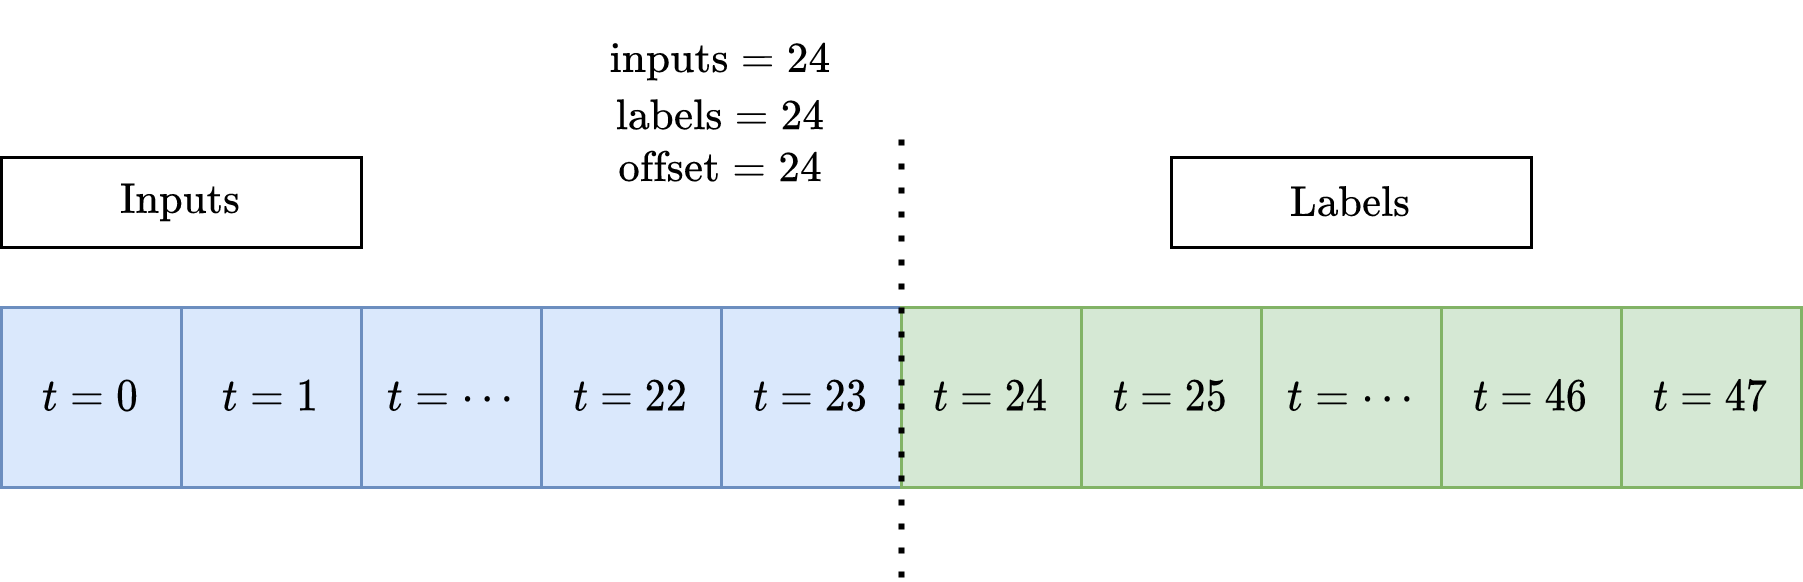
\includegraphics[width=12cm]{images/solution/modules/windows/windows-1.png}
    \caption{Ventana con un múltiples entradas y múltiples salidas}
\end{figure}


\begin{figure}[H]
    \centering
    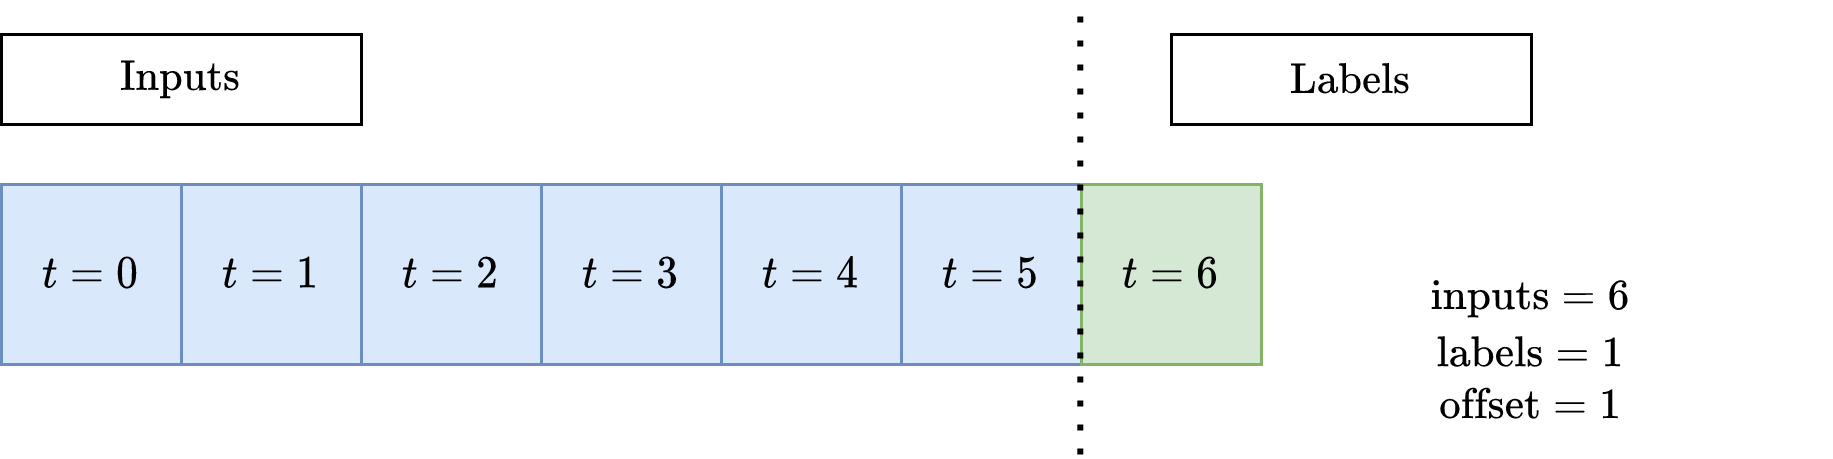
\includegraphics[width=12cm]{images/solution/modules/windows/windows-2.png}
    \caption{Ventana con un único intervalo de salida}
\end{figure}



\begin{figure}[H]
    \centering
    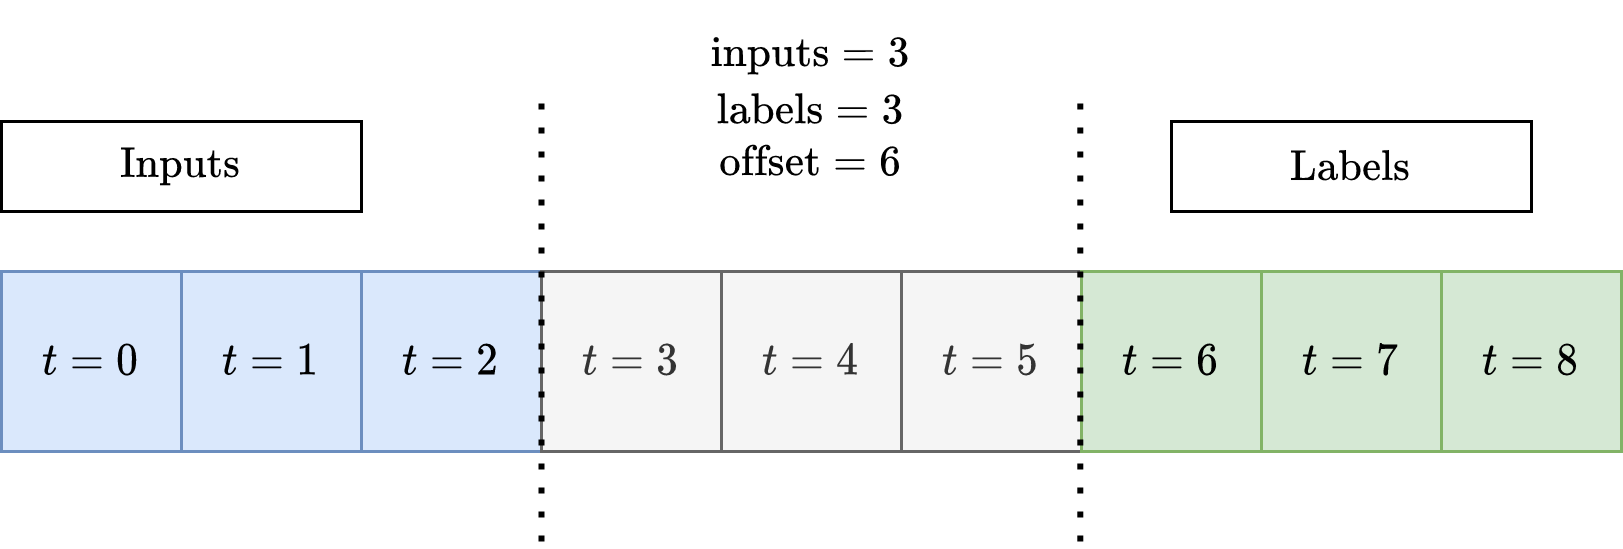
\includegraphics[width=12cm]{images/solution/modules/windows/windows-3.png}
    \caption{Ventana con \textit{offset}}
\end{figure}

Las cajas representan intervalos. El color azul representa que serán intervalos que el modelo usará como de entrada, es decir, cada caja azul tiene asociado un vector con \textit{hour}, \textit{day\_of\_week}, \textit{month} y la cantidad de viajes iniciados para todas las estaciones en dicho intervalo. Esto, como se ha explicado en la sección \ref{inputs-outputs}, se transformará en un vector de una única dimensión. Las cajas verdes por otro lado representa los intervalos que la red va las redes neuronales van a predecir. Por cada intervalo se creará un vector con tantos elementos como estaciones haya en el sistema siendo cada valor la predicción para cada estación. Como se verá más adelante, en las redes se incluirá una capa que permite la transformación de un vector a una matriz con lo que se conseguirá que la salida de las redes neuronales sea una matriz, donde cada fila es un intervalo y cada columna es una estación y cuyos valores serán las predicciones.
\newline


Las predicciones por otro lado se pueden realizar de dos formas distintas:

\begin{itemize}
    \item Predicción única: Dado un conjunto de datos de entrada se realizarán todas las predicciones a partir de esos datos.
    
    \begin{figure}[H]
    \centering
    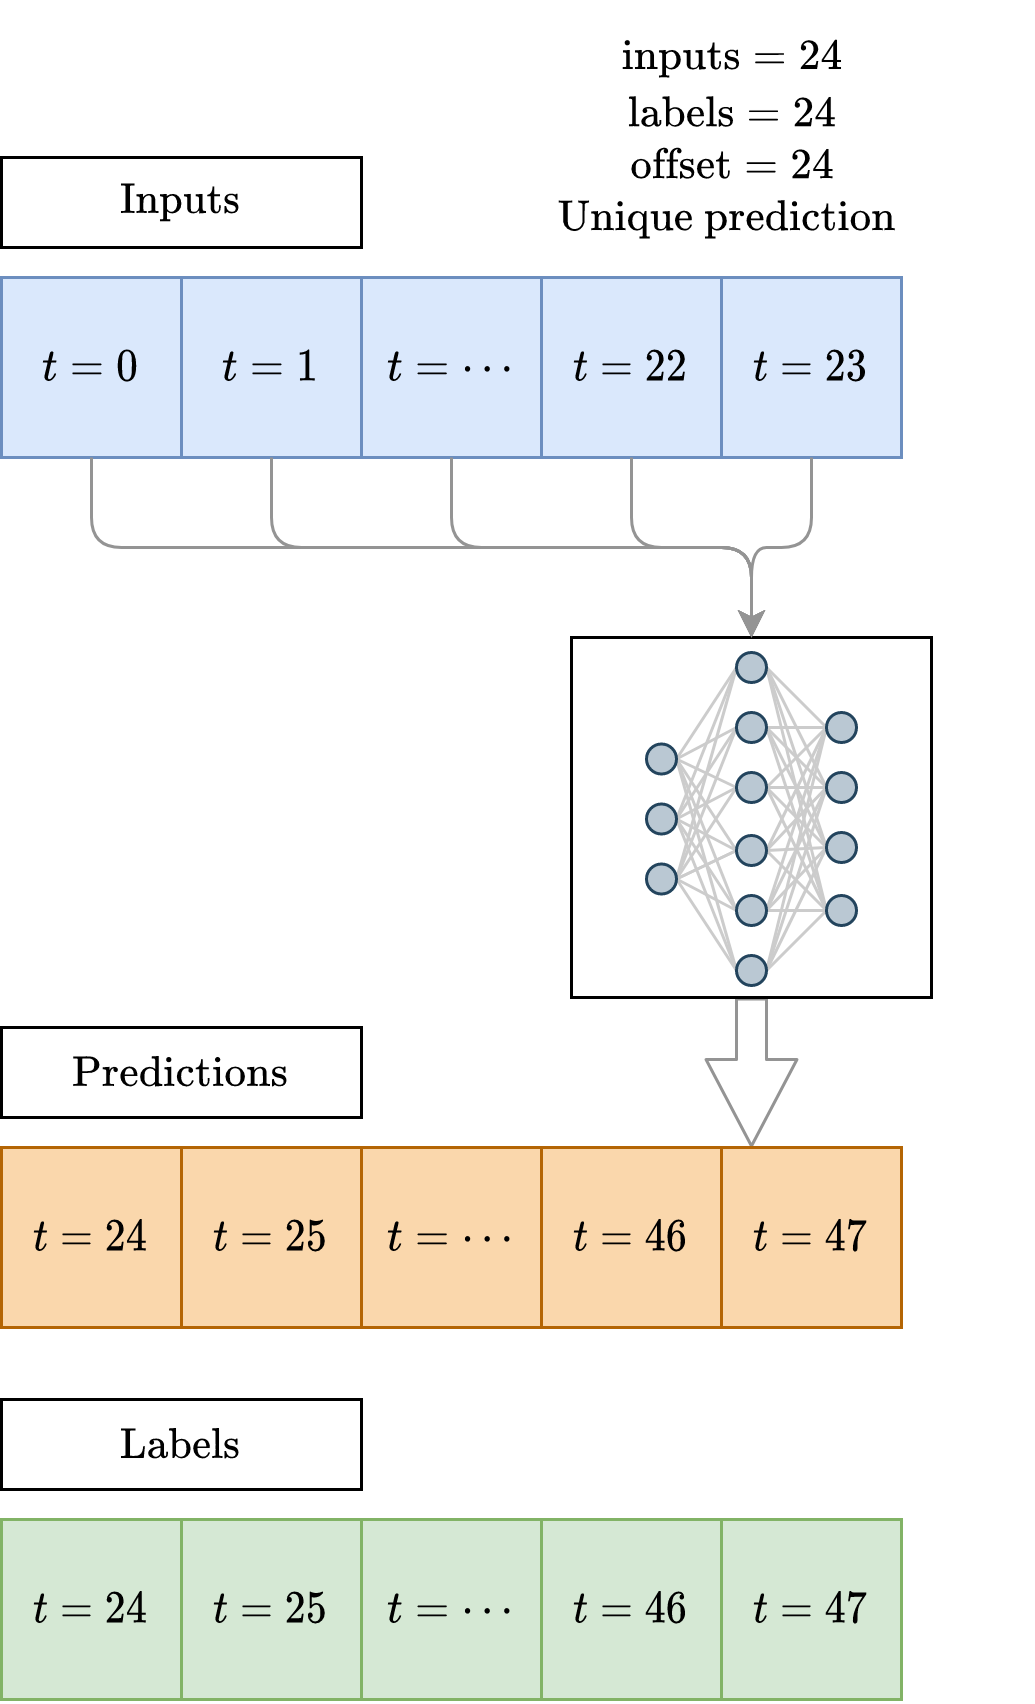
\includegraphics[width=7cm]{images/solution/modules/windows/windows-predictions-one-shot.png}
    \caption{Predicciones únicas}
    \end{figure}

    \item Predicción auto-regresiva \label{window_ar}: Se realizará primero la predicción más próxima en el futuro. Dicho valor será usado junto con el resto de valores de entrada (excepto el intervalo más pasado) para poder calcular la siguiente predicción. Visto gráficamente:
    \begin{figure}[H]
    \centering
    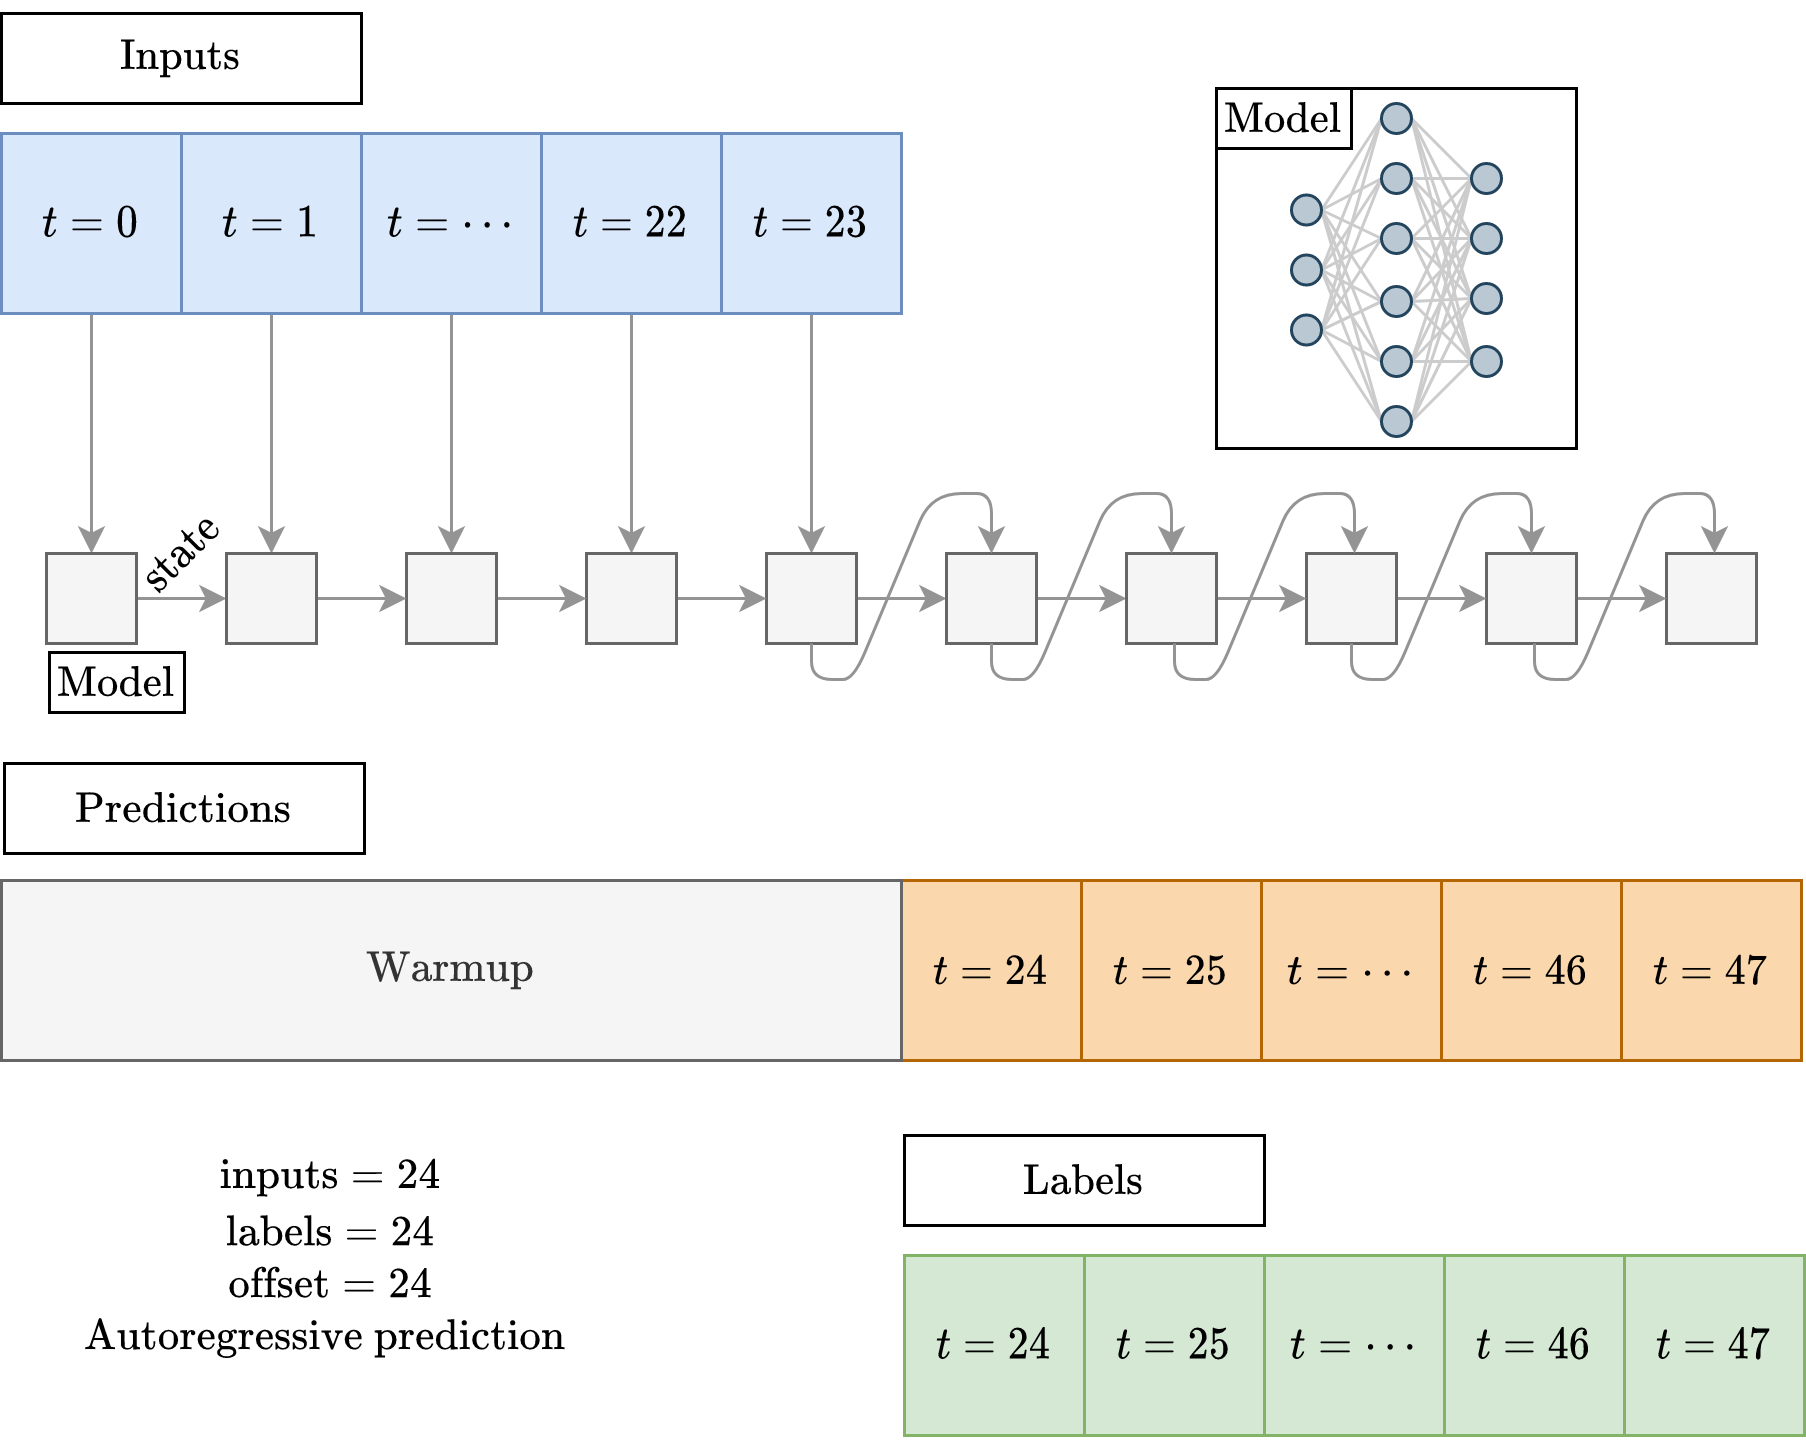
\includegraphics[width=12cm]{images/solution/modules/windows/windows-predictions-ar.png}
    \caption{Predicción auto-regresivas}
    \end{figure}
\end{itemize}

Una vez que se tengan las ventanas, hay que hacer que la ventana se pueda deslizar y de ese modo generar un nuevos vectores que servirán para el entrenamiento. Pongamos por ejemplo, que se dispone de un \textit{dataset} con 7 intervalos. Se quiere entrenar a un modelo que reciba 3 intervalos de entrada y 1 de salida. Por lo que el modelo se entrenará con un lote (\textit{batch}) de tamaño 4. Visto gráficamente, el funcionamiento de una ventana deslizante:

\begin{figure}[H]
    \centering
    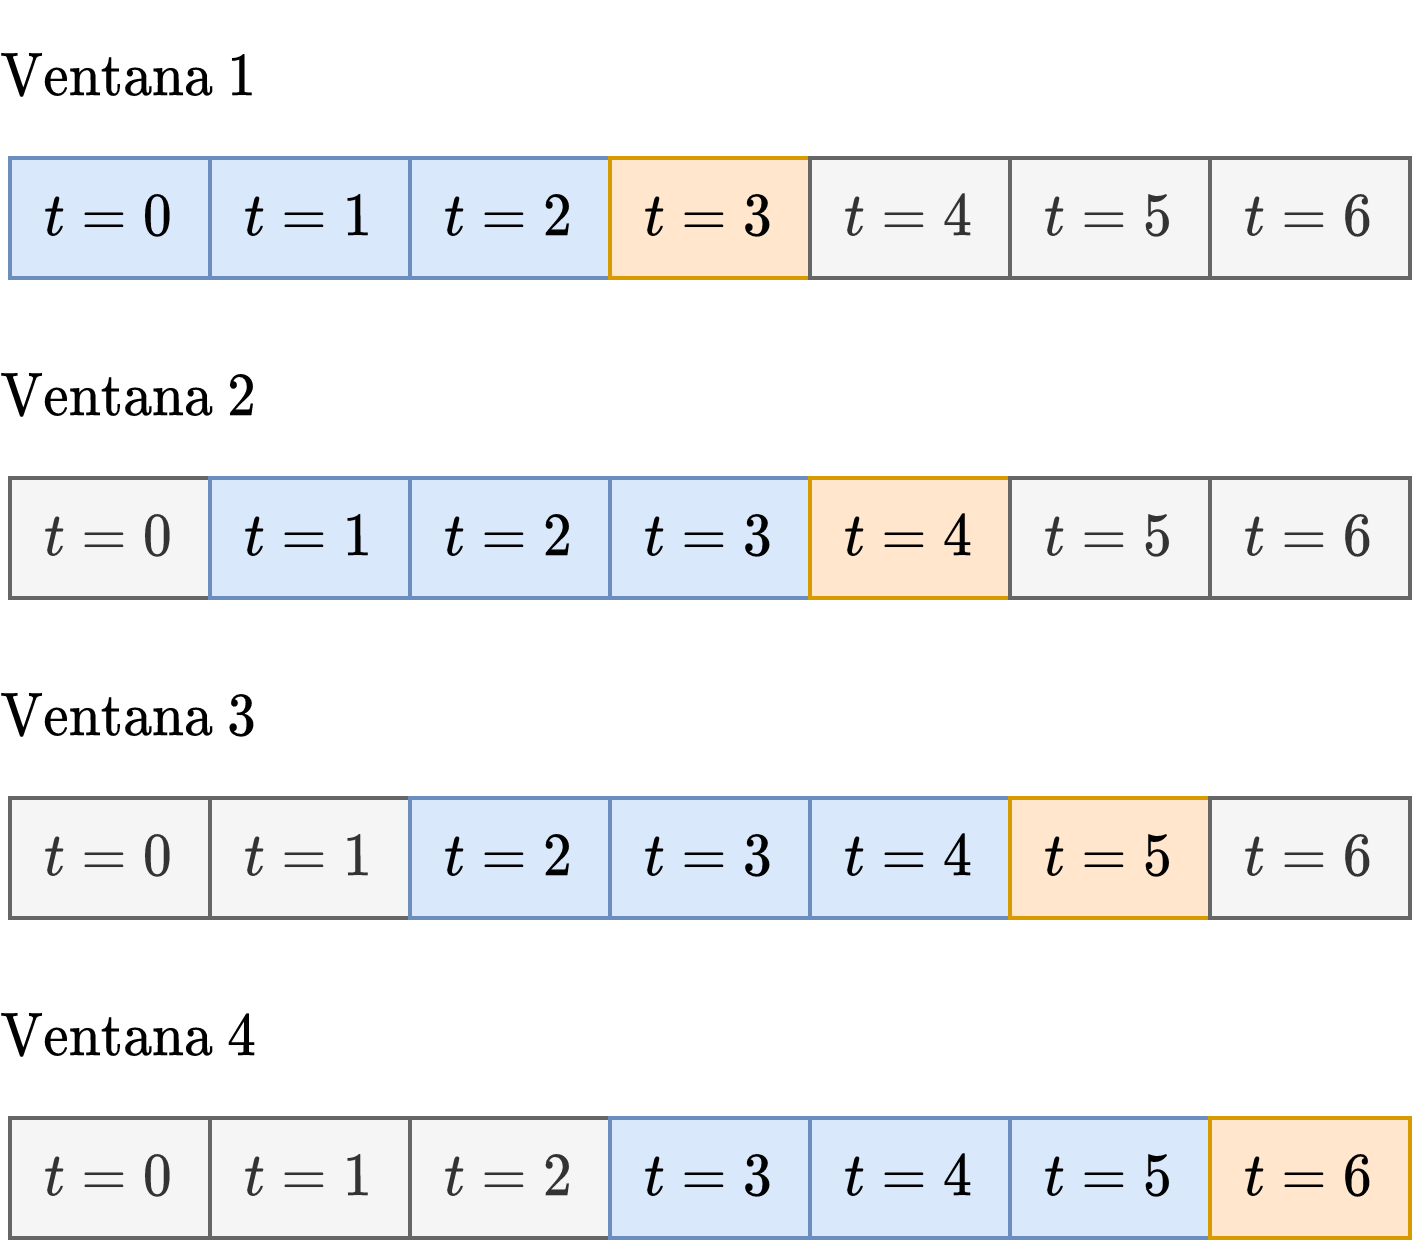
\includegraphics[width=7cm]{images/solution/modules/windows/sliding-windows.png}
    \caption{Funcionamiento de una ventana deslizante.}
\end{figure}


\subsubsection{Código del generador de ventanas}\label{window-generator-code}

Para este módulo se ha generado una clase que se encarga de crear objetos y se basa en gran parte en el tutorial oficial de \textit{Tensorflow} \cite{tensorflow2015-whitepaper} que ha sido modificado para suplir las necesidades del proyecto.
\newline

A continuación se van se explican todas los métodos usadas en la clase por partes.

\begin{itemize}
    \item Índices y \textit{offsets}:  El método \small{\verb|__init__|} (constructor en \textit{Python}) incluye toda la lógica necesaria para los índices de entrada y de etiqueta. También toma los \small{\verb|DataFrames|} de entrenamiento, validación y test como entrada. Estos serán convertidos a \small{\verb|tf.data.Datasets|} de ventanas más tarde. Por último, recibe el índice de la columna donde se encuentra la información temporal. Este índice es un valor igual a $-3$, pues como se puede ver en la tabla \ref{tab:intervals_example}, las tres últimas columnas son las que contienen información sobre la hora, día de la semana y mes.

\begin{minted}[fontsize=\scriptsize]{python}
import tensorflow as tf
import numpy as np


class WindowGenerator():
    def __init__(self, input_width, label_width, shift,
                 train_df, val_df, test_df=None,
                 label_columns_index=-3):

        # Store the datasets
        self.train_df = train_df
        self.val_df = val_df
        self.test_df = test_df

        # Gets the indexes of the label column.
        self.label_columns_index = label_columns_index
        self.label_columns = train_df.columns[:label_columns_index]
                                     .tolist()
        self.label_columns_indices = {name: i for i, name in
                                      enumerate(self.label_columns)}
    
        # Dict of name of column as key and index as value
        self.column_indices = {name: i for i, name in
                               enumerate(train_df.columns)}

        # Work out the window parameters.
        self.input_width = input_width
        self.label_width = label_width
        self.shift = shift
        
        # Handle the indexes and offsets as shown in the diagrams
        # above.
        self.total_window_size = input_width + shift

        self.input_slice = slice(0, input_width)
        self.input_indices = np.arange(self.total_window_size)[
            self.input_slice]

        self.label_start = self.total_window_size - self.label_width
        self.labels_slice = slice(self.label_start, None)
        self.label_indices = np.arange(self.total_window_size)[
            self.labels_slice]
\end{minted}

\item División de la ventana entre \textit{input} y \textit{label}: Dada una lista de intervalos consecutivas, el método \small{\verb|split_window()|} convertirá en una ventana de entradas y una ventana de etiquetas.

\begin{minted}[fontsize=\scriptsize]{python}
def split_window(self, features):
    inputs = features[:, self.input_slice, :]
    labels = features[:, self.labels_slice, :]

    if self.label_columns is not None:
        labels = tf.stack(
            [labels[:, :, self.column_indices[name]]
                for name in self.label_columns],
            axis=-1)

    # Slicing doesn't preserve static shape information, so set
    # the shapes manually. This way the `tf.data.Datasets` are
    # easier to inspect.
    inputs.set_shape([None, self.input_width, None])
    labels.set_shape([None, self.label_width, None])
    return inputs, labels
\end{minted}


\item Creación de los \small{\verb|tf.data.Datasets|}: Finalmente este método small{\verb|make_dataset()|} tomará un \small{\verb|DataFrame|} de intervalos y lo convertirá en un \small{\verb|tf.data.Dataset|} de pares (\small{\verb|input_window|}, \small{\verb|label_window|}). Y como se puede ver a continuación se han creado \textit{batches} de tamaño $32$.


\begin{minted}[fontsize=\scriptsize]{python}
def make_dataset(self, data):
    if data is None:
        print("Data is None")
        return

    data = np.array(data, dtype=np.float32)
    ds = tf.keras.preprocessing.timeseries_dataset_from_array(
        data=data,
        targets=None,
        sequence_length=self.total_window_size,
        sequence_stride=1,
        shuffle=True,
        batch_size=32,)

    ds = ds.map(self.split_window)

    return ds
\end{minted}

\item La clase \small{\verb|WindowGenerator|} contiene los \small{\verb|DataFrame|} de entrenamiento, validación y test. Por lo que al final, se añaden las propiedades para acceder a ellos que son de tipo \small{\verb|tf.data.Datasets|} usando el método anterior \small\verb|make_dataset|:
\begin{minted}[fontsize=\scriptsize]{python}
@property
def train(self):
  return self.make_dataset(self.train_df)

@property
def val(self):
  return self.make_dataset(self.val_df)

@property
def test(self):
  return self.make_dataset(self.test_df)
\end{minted}
\end{itemize}